\section{Summary of Paper \ref{pap:daiyong}}
\subsection*{"\nameref{pap:daiyong}"}
Least Square Support Vector Regression (LS-SVR) \cite{brereton_support_2010} is used in Paper \ref{pap:daiyong} to identify the parameters in the AVMM.  
The data is taken from experimental tests on a lake using a ship model with a scale of 50:1. The configuration of sensors and equipment for the experiment is shown in Fig.\ref{fig:cthmodel}.  
\begin{figure}[H]
    \centering
    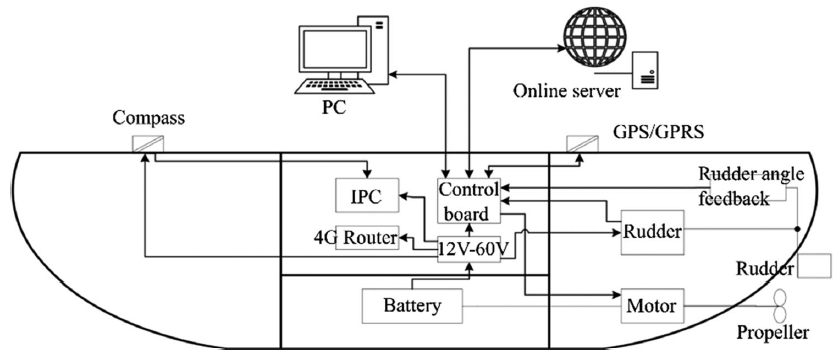
\includegraphics[width=\textwidth]{kappa/images/cth_model.png}
    \caption{Configuration of sensors and equipment for the experimental tests.}
    \label{fig:cthmodel}
\end{figure}
\noindent The hydrodynamic derivatives of the AVMM are identified almost perfectly when applied on data from simulations with MSS toolbox Mariner \cite{tristan_matlab_2009}. The  does however not work at all when applied on the data obtained from the lake experiments as seen in Fig.\ref{fig:daiyong_extrapolation}. 

\begin{figure}[H]
    \centering
    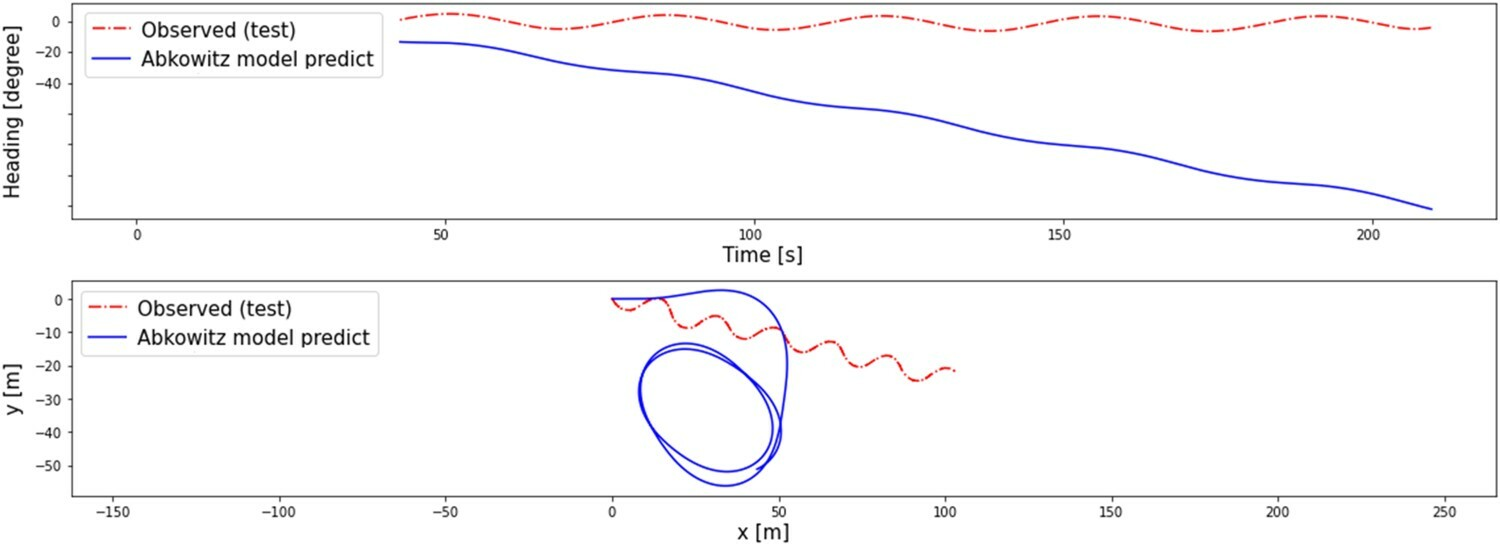
\includegraphics[width=\linewidth]{kappa/images/daiyong_extrapolation.jpeg}
    \caption{Prediction with AVMM of zigzag lake experiments.}
    \label{fig:daiyong_extrapolation}
\end{figure}

\noindent The  is very sensitive to noise due to the differentiation that needs to be conducted to calculate velocities and yaw rate from the measured position and heading. The  works better if the data is first cleaned using a proposed preprocessing algorithm together with a Kalman Filter (KF). The simulations with the identified model and the experiments were however still not in very good agreement.  